
\begin{frame}{Multicontact Locomotion}
\vspace*{-0.5cm}
\begin{itemize}
 \item Observation : Great energy consumption during climbing stairs
\end{itemize}

\begin{center}
  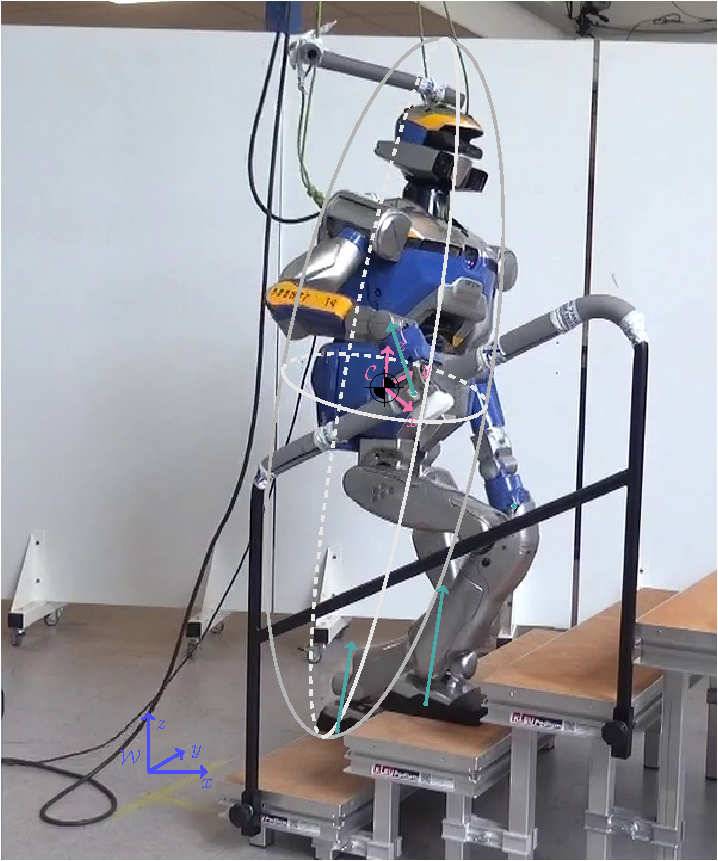
\includegraphics[height=0.6\textheight]{multicontact/cover.pdf}
  \hspace*{0.5cm}
  \begin{minipage}{0.3\linewidth}
    \vspace*{-4.8cm}
    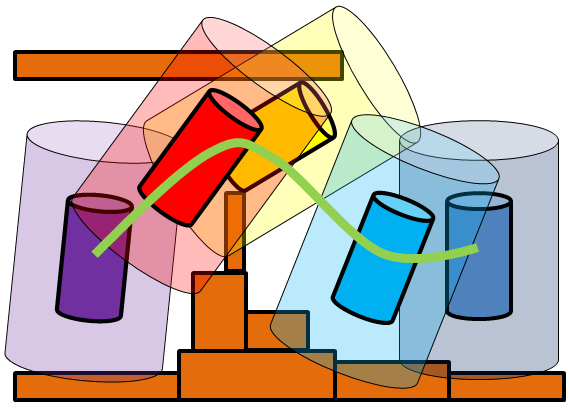
\includegraphics[width=\linewidth]{multicontact/rbprm2.png}\\
    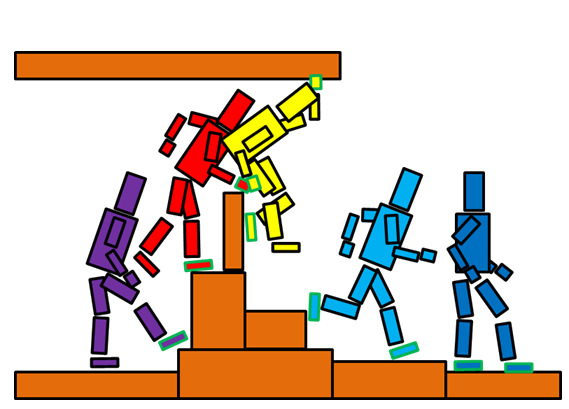
\includegraphics[width=\linewidth]{multicontact/rbprm3.png}  
  \end{minipage}
\end{center}


\begin{itemize}
 \item Hypothesis : Distributing the forces on the whole robot body will decrease the energy consumption
\end{itemize}

\end{frame}

%%%%%%%%%%%%%%%%%%%%%%%%%%%%%%%%%%%%%%%%%%%%%%%%%%%%%%%%%%%%%%%%%%%%%%%%%%%%%%%


\begin{frame}{Centroidal Dynamics}

\begin{itemize}

\item The dynamic constraint \textcolor{txtcolor2}{(M. Kudruss, Humanoids 2015)} :
\begin{scriptsize}
\begin{align*}
  m
  \begin{bmatrix}
  \ddcom - {\bf g} \\
  \com \times (\ddcom - {\bf g})
  \end{bmatrix}
  +
  \begin{bmatrix}
   {\bf 0} \\
     \textcolor{txtcolor2}{{\bf I}_c \dot{\omega}}
  \end{bmatrix}
  =
  \begin{bmatrix}
  \sum_{i=1}^{M}
  \Qf \ff \\
  \sum_{i=1}^{M}
  \pf \times \Qf  \ff
  \end{bmatrix}
\end{align*}
\end{scriptsize}
\item the state :
$
\begin{bmatrix}
\com & \dcom & \textcolor{txtcolor2}{\omega}
\end{bmatrix}^T
$
\item the controls :
$
\begin{bmatrix}
\ff
\end{bmatrix}^T
$

\textcolor{txtcolor1}{\hrule}
\vspace*{0.5cm}

\item The dynamic constraint \textcolor{txtcolor5}{(J. Carpentier, ICRA 2016)} :
\begin{scriptsize}
\begin{align*}
  m
  \begin{bmatrix}
  \ddcom - {\bf g} \\
  \com \times (\ddcom - {\bf g})
  \end{bmatrix}
  +
  \begin{bmatrix}
   {\bf 0} \\
   \textcolor{txtcolor5}{ \dot{\bf \am} }
  \end{bmatrix}
  =
  \begin{bmatrix}
  \sum_{i=1}^{M}
  \Qf \ff \\
  \sum_{i=1}^{M}
  \pf \times \Qf  \ff +
  \textcolor{txtcolor5}{ \Qf \tauf}
  \end{bmatrix}
\end{align*}
\end{scriptsize}
\item the state :
$
\begin{bmatrix}
\com & {\bf h}=m\dcom & \textcolor{txtcolor5}{\mathcal{L}}
\end{bmatrix}^T
$
\item the controls :
$
\begin{bmatrix}
\ff & \textcolor{txtcolor5}{\tauf}
\end{bmatrix}^T
$

\end{itemize}

\end{frame}

%%%%%%%%%%%%%%%%%%%%%%%%%%%%%%%%%%%%%%%%%%%%%%%%%%%%%%%%%%%%%%%%%%%%%%%%%%%%%%%

\begin{frame}{The optimal control problem}
\vspace*{-0.5cm}
\begin{columns}
\begin{column}{0.5\textwidth}

\begin{itemize}
  \item {(M. Kudruss, Humanoids 2015)}
\end{itemize}

\begin{itemize}
  \item Cost Functions :
  \begin{itemize}
    \item Linear/Angular velocity
    \item \textcolor{blue!70!black}{CoM attracted by all contacts}
    \item Controls (forces)
    \item \textcolor{blue!70!black}{Fixed sequence timing}
    \item Linear/Angular acceleration
  \end{itemize}
  \vspace*{0.5cm}
  \item Constraints :
  \begin{itemize}
    \item \textcolor{blue!70!black}{Kinematic Constraints}
    \item \textcolor{blue!70!black}{3D Friction Cone}
  \end{itemize}
\end{itemize}
%
%\begin{subequations}
%\begin{eqnarray*}
%\hspace{0em}	\underset{\substack{\hspace{0.2em} \underline{\bm x}, \; \underline{\bm u}} }{\min } \ \ \
%	& & \hspace{-4em} \int_{0}^{T}
%%	{\scriptstyle
%	  \textcolor{red!70!black}{||\dcom||^2_2 +
%	  ||{\omega}||^2_2} +
%    \textcolor{orange!70!black}{\ell_2\,_{kin}} \\
%    & & \hspace{-3em} +
%    \textcolor{green!50!black}{||{\dot{\omega}}||^2_2} +
%    \textcolor{purple!100!blue!100}{||{\ddcom}||^2_2}
%%  }
%  dt  \\[1em]
%	s.t.
%	&  \forall t,i& \ff \in \mathcal{K}_i^{\textcolor{blue!50!green!100!black}{3D}} \\
%  &  \forall t& \textcolor{orange!70!black}{\com ,\; \dcom} ,\; {\omega} \in \mathcal{B}_x \\ 
%  &  \forall t,i& {\ff ,\; {\sigma}} \in \mathcal{B}_u    \\[1em]
%  & \forall t & \dot{\bm{x}} = {dyn}(\bm x, \bm u)  \\	
%	& & \hspace{-4em} \bm x(0) = \bm x_{0} \; ; \; \bm x(T) \in \mathcal{X}_* 
%\end{eqnarray*}
%\end{subequations}

\end{column}
%
{\color{txtcolor2}\vrule}
%
%
\begin{column}{0.5\textwidth}

\begin{itemize}
\item {(J. Carpentier, ICRA 2016)}
\end{itemize}

\begin{itemize}
  \item Cost Functions :
  \begin{itemize}
    \item {Linear Momentum}
    \item \textcolor{blue!70!black}{CoM rejected by all contacts}
    \item {Controls (forces and torques)}
    \item \textcolor{blue!70!black}{Free sequence timing}
    \item {Linear/Angular momentum derivatives}
  \end{itemize}
  \item Constraints :
  \begin{itemize}
    \item \textcolor{blue!70!black}{No Kinematics Hard Constraints}
    \item \textcolor{blue!70!black}{6D Friction Cone}
  \end{itemize}
\end{itemize}

%
%\begin{subequations}
%\begin{eqnarray*}
%\hspace{0em}	\underset{\substack{\hspace{0.2em} \underline{\bm x}, \; \underline{\bm u}} }{\min } \ \ \  
%	& & \hspace{-4em} \int_{0}^{T}
%%	{\scriptstyle
%    \textcolor{red!70!black}{||m\dcom||^2_2} +
%  	  \textcolor{orange!70!black}{\text{exp}_{kin}} \\
%  	  & & \hspace{-3em} +
%    \textcolor{green!50!black}{||{\dot{\mathcal{L}}}||^2_2} +
%	  \textcolor{purple!100!blue!100}{||{\ff}||^2_2} +
% 	  \textcolor{purple!100!blue!100}{||{\tauf}||^2_2} 
%%  }
%  dt  \\[1em]
%	s.t.
%	&  \forall t,i& [\ff \;\; {\tauf}] \in \mathcal{K}_i^{\textcolor{blue!50!green!100!black}{6D}} \\
%  &  \forall t& {{\mathcal{L}}} \in \mathcal{B}_{\mathcal{L}}    \\ 
%  &  \forall t& {\ff ,\; {\tauf}} \in \mathcal{B}_u    \\ [1em]
%  & \forall t,i & \dot{\bm{x}} = {dyn}(\bm x, \bm u)  \\	
%	& & \hspace{-4em} \bm x(0) = \bm x_{0} \; ; \; \bm x(T) \in \mathcal{X}_* 
%\end{eqnarray*}
%\end{subequations}

\end{column}
\end{columns}


\end{frame}

%%%%%%%%%%%%%%%%%%%%%%%%%%%%%%%%%%%%%%%%%%%%%%%%%%%%%%%%%%%%%%%%%%%%%%%%%%%%%%%

\begin{frame}{Experiment on HRP2}
  \begin{center}
    \movie[autostart,loop]{
    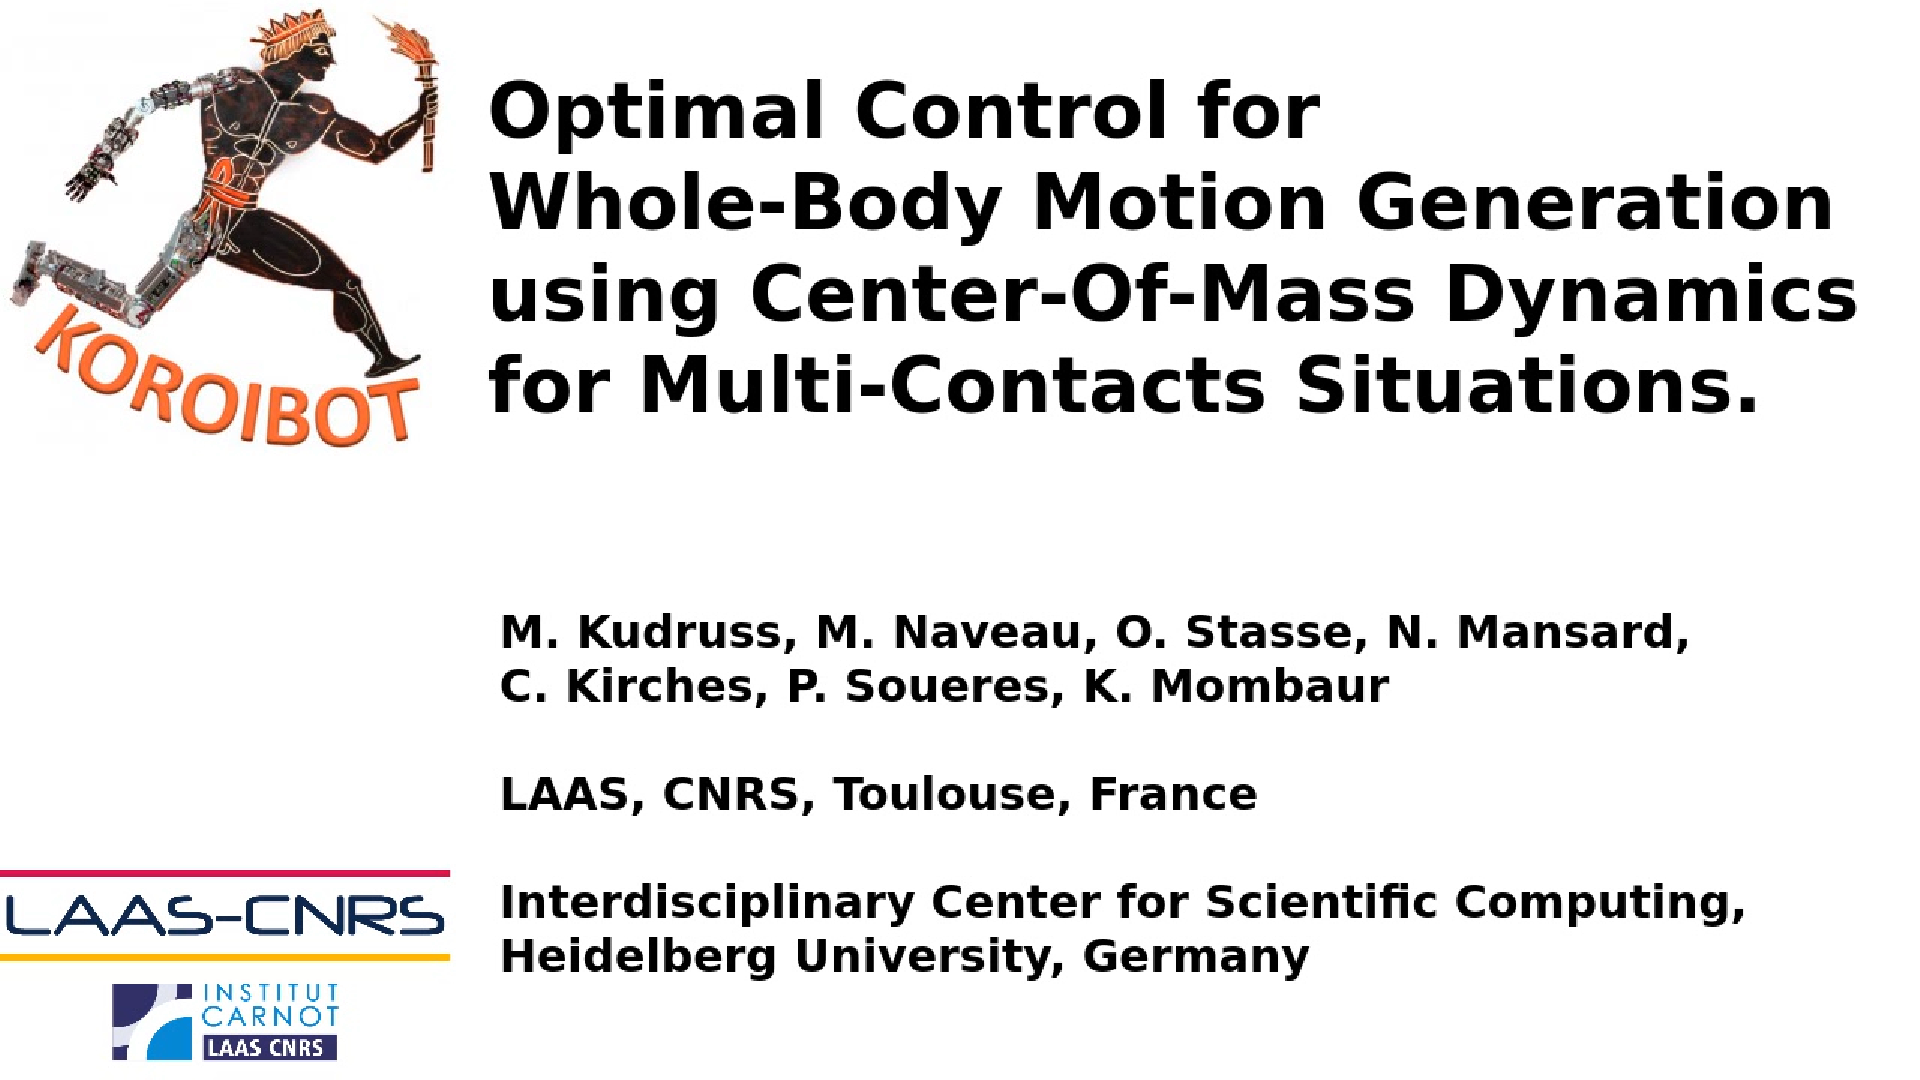
\includegraphics[width=0.8\linewidth, keepaspectratio]
      {multicontact/15-ichr-multicontact.png}
    }  
    {videos/multicontact-short.mp4}
  \end{center}
  \vspace*{-0.5cm}
  \blfootnote{Kudruss, \textbf{Naveau} et al. Humanoids 2015)}
  \blfootnote{Carpentier, Tonneau, \textbf{Naveau} et al. ICRA 2016)}
\end{frame}

%%%%%%%%%%%%%%%%%%%%%%%%%%%%%%%%%%%%%%%%%%%%%%%%%%%%%%%%%%%%%%%%%%%%%%%%%%%%%%%



%\begin{equation}
%  m
%  \begin{bmatrix}
%  \ddcom - {\bf g} \\
%  \com \times (\ddcom - {\bf g})
%  \end{bmatrix}
%  +
%  \begin{bmatrix}
%  {\bf 0} \\
%  \tikz[baseline]{
%      \node[anchor=base] (l) {$ \dot{\mathcal{L}} $} ;
%      %
%      \draw [draw,-,color=red!50,thick] ([xshift=-0.2cm,yshift= 0.2cm]l.center) -- node {}     ([xshift= 0.2cm,yshift=-0.2cm]l.center);
%      %
%      \draw [draw,-,color=red!50,thick] ([xshift=-0.2cm,yshift=-0.2cm]l.center) -- node {}     ([xshift= 0.2cm,yshift= 0.2cm]l.center);
%    }
%  \end{bmatrix}
%  =
%  \begin{bmatrix}
%  \sum_{i=1}^{M}
%  \Qf \ff \\
%  \sum_{i=1}^{M}
%  \pf \times \Qf  \ff
%  \end{bmatrix}
%\end{equation}